\chapter{Helpful Rules and Tricks for Resistor Circuits}
\label{chap:resistorRulesAndTricks}
In this chapter, I'll finalize some terminology we'll use a lot in this course, and then we're going to use the laws we saw in Chapter \ref{chap:fundamentals} to derive some rules that will simplify the process of analyzing circuit behavior. The rules and tricks derived in this chapter can help you see past the density of elements in some circuits to discern their underlying functionality. Furthermore, even though we are working in the context of resistors exclusively, the applicability of this material extends to all passive elements (resistors, capacitors, and inductors), which we will see later in the course.
 
\section{Circuit Terminology}
Before we proceed, I need to introduce some circuit concepts. I will use these terms from now on, so it's important that we all know what they mean.
\begin{figure}[h!]
\centering
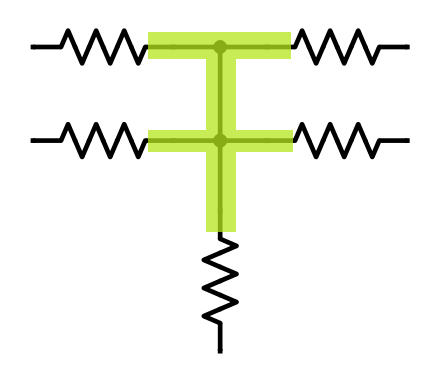
\includegraphics[width=13cm]{figures/nodeCloseUp.png}
\caption{The highlighted common connection that these resistors share is an example of a \textit{node}.}
\label{nodeCloseUp}
\end{figure}
\par
I introduced \textbf{nodes} in Chapter \ref{chap:fundamentals}, but their definition bears repeating and expanding; a \textbf{node} is a place in a circuit where two or more elements are connected. An example of a node is highlighted in Figure \ref{nodeCloseUp}. At any node, there is just one voltage value. All the nodes of the circuit in Figure \ref{nodesHighlighted} have been highlighted. You can see that nodes can be simple or elaborate in shape, but being able to determine how many nodes are in a circuit is an important skill.
\begin{figure}[h!]
\centering
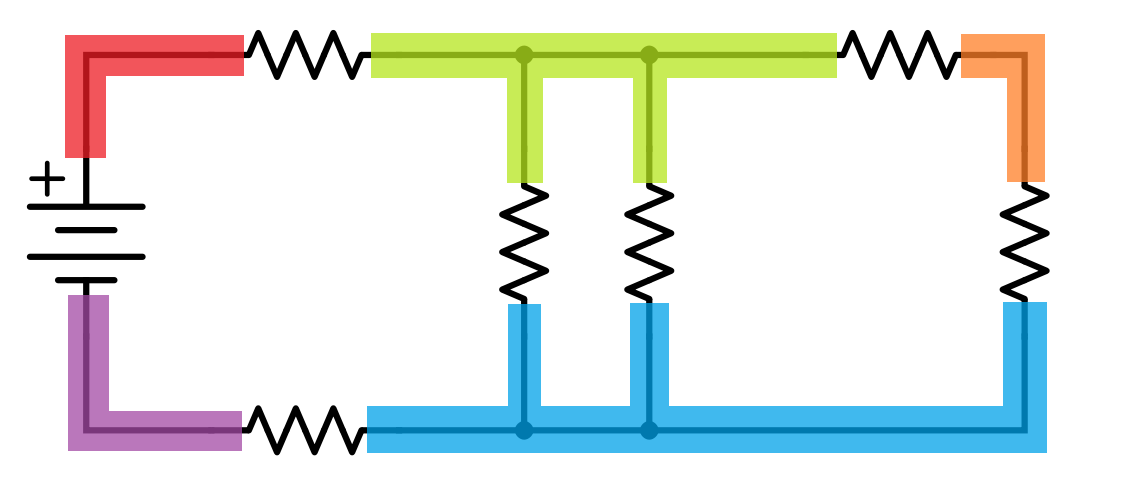
\includegraphics[width=13cm]{figures/nodesHighlighted.png}
\caption{The nodes in this circuit are each highlighted in a different color.}
\label{nodesHighlighted}
\end{figure}

\par
A \textbf{branch} is simply a connection that allows current to flow between nodes. Branches are comprised of circuit elements like resistors and power supplies. The branches of the circuit in Figure \ref{branchesHighlighted} are highlighted. When I use the term \textbf{branch}, I mean a single path for current to flow through, and one branch could be comprised of several elements depending on the context. For example, in Figure~\ref{branchesHighlighted}, the leftmost three elements of the circuit together comprise a branch. Similarly, the rightmost two resistors in Figure~\ref{branchesHighlighted} comprise another branch.
\begin{figure}[h!]
\centering
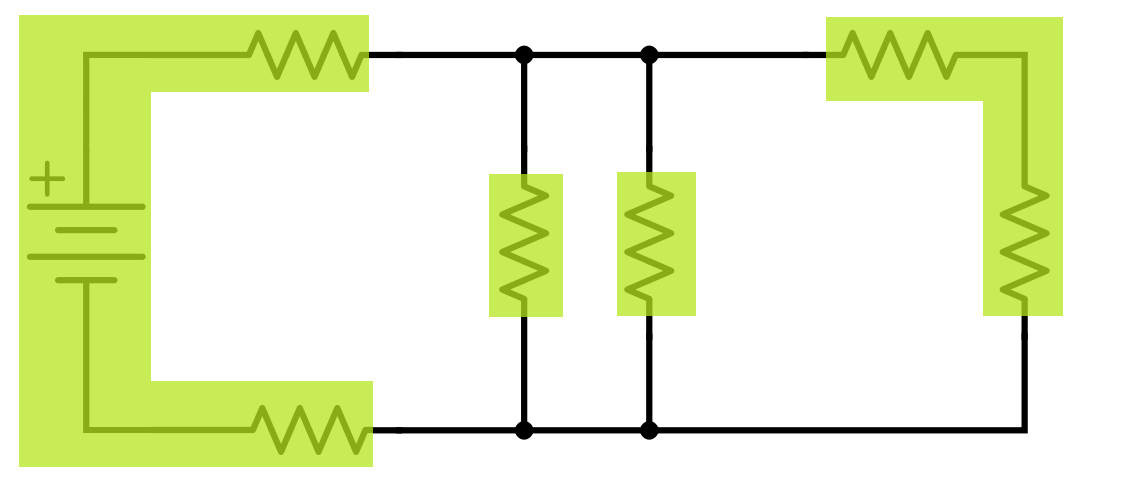
\includegraphics[width=13cm]{figures/branchesHighlighted.png}
\caption{The branches in this circuit are each highlighted.}
\label{branchesHighlighted}
\end{figure}

\par
If I describe several elements as being \textbf{in series}, that means that there is a single path for current to flow through them; in other words, they are connected head-to-tail, with only two elements sharing each node in the series connection. Two resistors in series have been highlighted in the circuit of Figure \ref{seriesHighlighted}. There is only one path for current to flow through those two elements, and there are no other branches connected to their shared node.
\begin{figure}[h!]
\centering
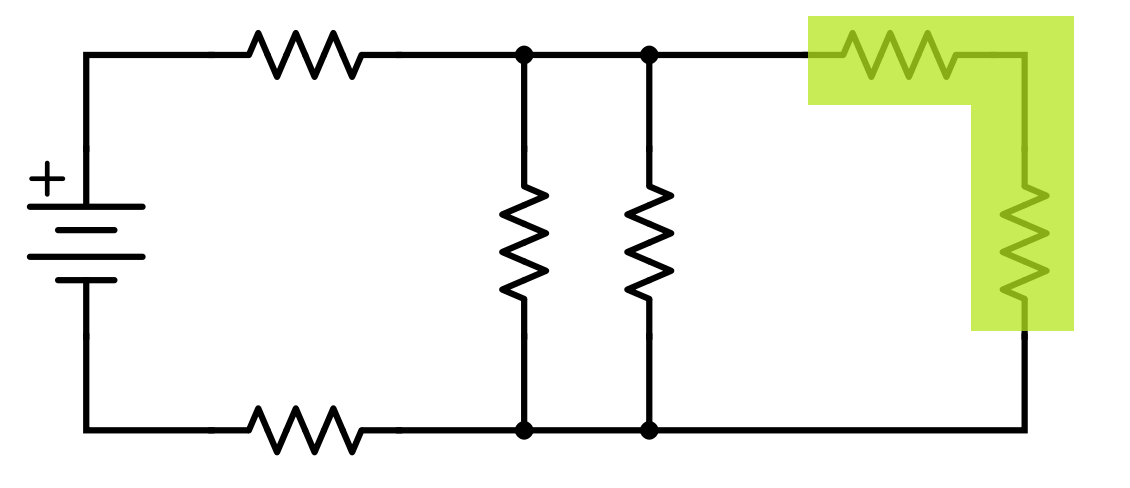
\includegraphics[width=13cm]{figures/seriesHighlighted.png}
\caption{The two highlighted resistors in this circuit are in series.}
\label{seriesHighlighted}
\end{figure}
\par
\textbf{Parallel} elements share both of their nodes with each other. Two parallel resistors are highlighted in the circuit of Figure \ref{parallelHighlighted}. We know these resistors are in parallel because they share both of their nodes.
\begin{figure}[h!]
\centering
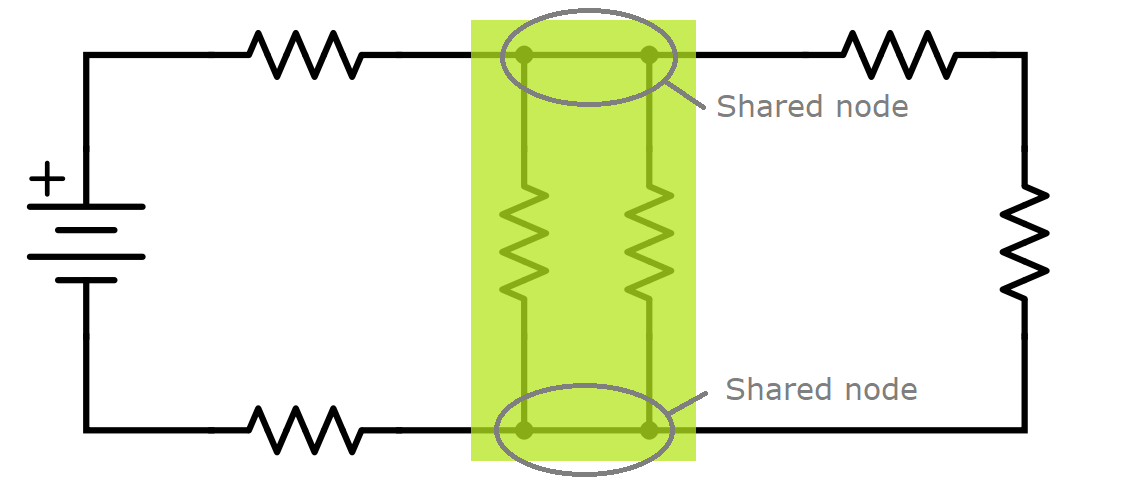
\includegraphics[width=13cm]{figures/parallelHighlighted.png}
\caption{The two highlighted resistors in this circuit are in parallel. We can tell this, because their head and tail nodes are shared.}
\label{parallelHighlighted}
\end{figure}
\par
Now that we have defined these terms, it's time to learn some rules and tricks for simplifying circuit analysis.

\section{Using Ohm's Law to Define Resistance}
Ohm's Law states that the voltage across a resistor is equal to to the value of the current flowing through that resistor multiplied by its resistance ($V = i \cdot R$). From this law, we could also define resistance of any general circuit element or collection of elements in a circuit as the ratio of the voltage across it divided by the current flowing through it, as shown in Figure \ref{genericElementResistance}. 
\begin{figure}[h!]
\centering
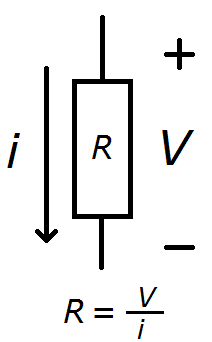
\includegraphics[width=3cm]{figures/singleElementRes.png}
\caption{The resistance of a circuit element or a collection of elements is defined as $R = V/i$ according to Ohm's law.}
\label{genericElementResistance}
\end{figure}

The circuits we have seen so far have had just a single resistor, but most real circuits have dozens or more. Any grouping of resistors can be simplified by finding an equivalent resistance for the entire collection.


\section{Equivalent Resistance of Series Resistors}
\label{sec:seriesEquivalent}
Let's consider a section of a circuit comprised of two resistors connected in series like that shown in Figure \ref{twoSeriesToEquivalent}. If we want to simplify a series of resistances like this into a single equivalent resistance, all we need to do is determine the value of the current flowing  through the resistors and then calculate the ratio of the voltage across them ($V_s$ in this case) to that current. 
\begin{figure}[h!]
\centering
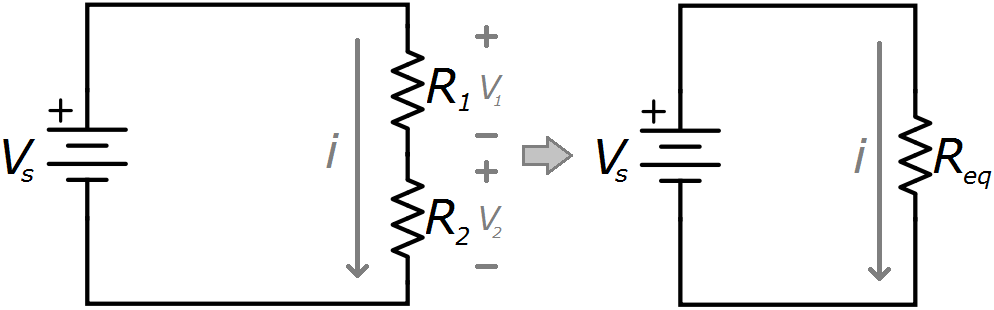
\includegraphics[width=13cm]{figures/twoResSeries.png}
\caption{The current flowing through two resistors in series and the voltage across both define their equivalent resistance.}
\label{twoSeriesToEquivalent}
\end{figure}
We can relate the voltage drops across each resistor (which I have labelled $V_1$ and $V_2$) and the source voltage using Kirchhoff's Voltage Law: $V_s = V_1 + V_2$. We can further define $V_1$ and $V_2$ in terms of the current flowing through the branch, $i$ and the respective resistances as $V_1 = i \cdot R_1$ and $V_2 = i \cdot R_2$. We also know that the current flowing through each resistor is the same, and we can define it as $i = \frac{V_s}{R_{eq}}$. Putting these expressions together and manipulating them algebraically yields the following:
$$
i = \frac{V_1 + V_2}{R_{eq}} = \frac{i \cdot R_1 + i \cdot R_2}{R_{eq}} = \frac{i(R_1+R_2)}{R_{eq}}
$$
$$
\textrm{     therefore     }R_{eq} = \frac{\bcancel{i}(R_1+R_2)}{\bcancel{i} \cdot R_{eq}} = R_1 + R_2
$$

Therefore, the equivalent resistance for the series of resistors $R_1$ and $R_2$ is given by their sum. This is the simplest specific case of the general rule for combining resistors in series:
$$
\textnormal{For any series of resistors    } R_1, R_2,\dots, R_n, \textnormal{   }R_{eq} = \sum_{i=1}^n{R_i}
$$
%parallel
\section{Equivalent Resistance of Parallel Resistors}
\label{sec:parallelResistors}
We can also calculate the equivalent resistance of parallel resistors. A pair of parallel resistors is shown in Figure \ref{twoParallelToEquivalent}. 
\begin{figure}[h!]
\centering
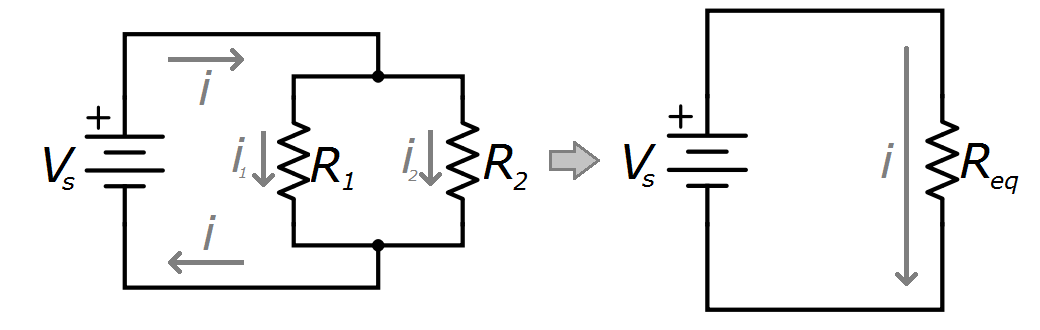
\includegraphics[width=13cm]{figures/twoResParallel.png}
\caption{Current flowing into two resistors in \textit{parallel} (i.e., sharing both head and tail nodes) and the voltage across them define their equivalent resistance.}
\label{twoParallelToEquivalent}
\end{figure}
This time, to determine the expression for $R_{eq}$, we will first use Kirchhoff's Current Law to relate $i$, the current coming from the source, to the labelled currents $i_1$ and $i_2$: 
$$i = i_1 + i_2$$
We know this is true, because current entering a node must be equal to the current leaving a node, and at the node above resistors $R_1$ and $R_2$, $i$ enters from the top, and $i_1$ and $i_2$ flow down through $R_1$ and $R_2$.
\par
Next, because these resistors share their head and tail nodes, we know that the voltage across $R_1$ is equal to the voltage across $R_2$. Furthermore, since $V_s$ is connected across both resistors, we know that the voltage across each resistor is just $V_s$. We can use this fact along with Ohm's Law to determine expressions for $i_1$ and $i_2$:
$$
V_s = i_1\cdot R_1\textnormal{, so   }i_1 = \frac{V_s}{R_1}
$$
and similarly
$$
i_2 = \frac{V_s}{R_2}
$$
Combining these expressions for current with  the expressions above and the fact that $R_{eq} = \frac{V_s}{i}$ yields the following:
$$
R_{eq} = \frac{V_s}{i_1 + i_2} = \frac{V_s}{\frac{V_s}{R_1} + \frac{V_s}{R_2}} = \frac{\bcancel{V_s}}{\bcancel{V_s}\cdot(\frac{1}{R_1} + \frac{1}{R_2})} = \frac{1}{\frac{1}{R_1} + \frac{1}{R_2}}
$$
In general, for parallel resistors $ R_1, R_2,\dots, R_n,$ 
$$
R_{eq} = \frac{1}{\displaystyle\sum_{i=1}^n{\left(\frac{1}{R_i}\right)}}
$$
\par
In the special case of just two resistors in parallel---$R_1$ and $R_2$ in our example---we can always use the equivalent resistance
$$
R_{eq} = \frac{R_1R_2}{R_1+R_2}
$$
which is a convenient expression to remember.

%Voltage divider rule
\section{Voltage Dividers}
\label{sec:voltageDividers}
\begin{figure}[h!]
\centering
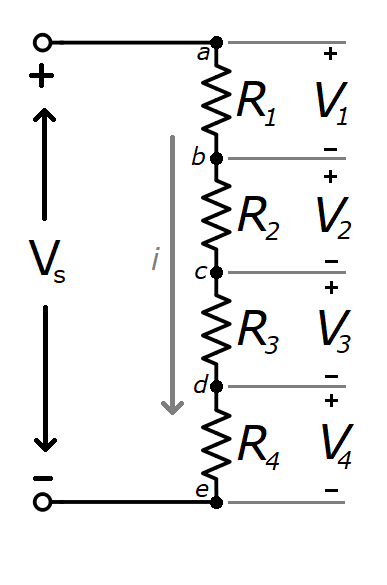
\includegraphics[width=5cm]{figures/voltageDivider.png}
\caption{These resistors in series form a voltage divider; they divide the voltage $V_s$ into four smaller voltages.}
\label{voltageDivider}
\end{figure}
Many circuits use resistors in series to reduce a voltage by some amount or to divide a voltage into smaller voltages. Because of this, a series connection of resistors is referred to as a \textbf{voltage divider}. An example voltage divider is shown in Figure \ref{voltageDivider}, and it divides the voltage $V_s$ into the four voltages $V_1$, $V_2$, $V_3$, and $V_4$. The values of these four voltages can be determined in terms of $V_s$ and the resistances $R_1$, $R_2$, $R_3$, and $R_4$ using the \textbf{Voltage Divider Rule}, which we will derive now using Figure \ref{voltageDivider}.
\par
First, let's assume there is an unknown current, $i$, flowing through the resistors in Figure \ref{voltageDivider} from top to bottom. In terms of that current and the resistances, Ohm's law tells us that the voltages across the four resistors are defined as 
$$
V_1 = i \cdot R_1
$$
$$
V_2 = i \cdot R_2
$$
$$
V_3 = i \cdot R_3
$$
$$
V_4 = i \cdot R_4
$$
We want to get rid of the current $i$ in our definitions for these voltages, because $i$ was not initially given and we should always find expressions in terms of variables that were defined in the initial circuit. In this case, we want our definitions for the voltages across each of the resistors to be given in terms of just the resistances in the circuit.
\par
In section \ref{sec:seriesEquivalent}, we learned that the equivalent resistance of all of the series of resistors in this voltage divider can be expressed as $R_{eq}=R_1 + R_2 + R_3 + R_4$. Then, Ohm's law tells us that $V_s = i \cdot R_{eq}$, and we can therefore define $i$ in terms of $V_s$ and $R_{eq}$ in the follwing way: 
$$
i=\frac{V_s}{R_{eq}}
$$
Folding this representation of $i$ into the expressions for voltages across the resistors yields
$$
V_1 = V_s \cdot \left(\frac{R_1}{R_{eq}}\right)
$$
$$
V_2 = V_s \cdot \left(\frac{R_2}{R_{eq}}\right) 
$$
$$
V_3 = V_s \cdot \left(\frac{R_3}{R_{eq}}\right)
$$
$$
V_4 = V_s \cdot \left(\frac{R_4}{R_{eq}}\right)
$$

I hope from these expressions you detect the pattern. Each of these are manifestations of the \textbf{Voltage Divider Rule}, which can be used to determine the voltage across any resistor in a voltage divider (which is really just a series of resistors):
$$
\mathlarger{\mathlarger{\mathlarger{V_n = V_s}}} \cdot \left(\frac{R_n}{\displaystyle\sum_{i=1}^m{R_i}}\right)
$$
This rule follows from the fundamental concepts of Chapter \ref{chap:fundamentals} and it is extremely useful. Once you get comfortable with the voltage divider rule, you will start to see voltage dividers in most circuits you encounter. When we start looking at time-varying (AC) voltages, capacitors, and inductors, we will find even more uses for the voltage divider rule in defining circuit behavior.

%Current divider rule
\section{Current Dividers}
\label{sec:currentDividers}
Parallel configurations of resistors are sometimes referred to as current dividers. I don't find these as useful as voltage dividers, but they do crop up in many circuits. Like in the last section, we will focus on a specific circuit---that of Figure \ref{currentDivider}---to derive a general rule for analyzing these circuit configurations.
\begin{figure}[h!]
\centering
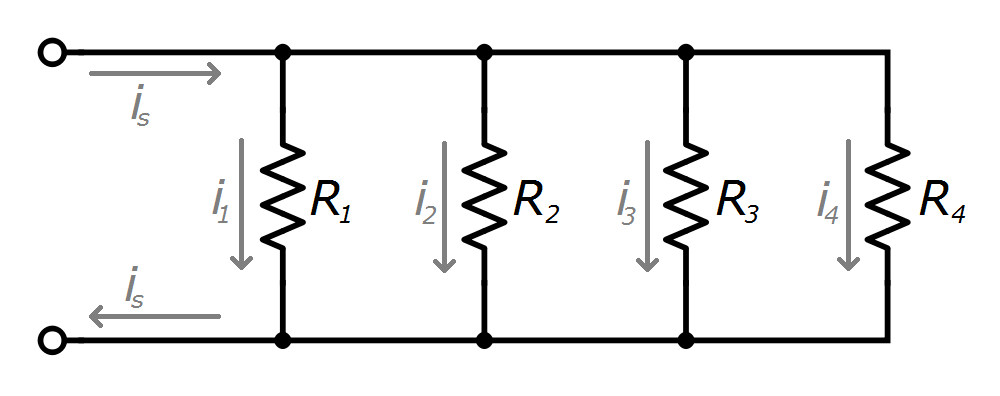
\includegraphics[width=10cm]{figures/currentDivider.png}
\caption{These resistors in parallel form a current divider; they divide the current $i_s$ into four smaller currents.}
\label{currentDivider}
\end{figure}
\par
Let's start off by assuming there is an unknown voltage $V$ across all four resistors in Figure \ref{currentDivider}. We can use that voltage and Ohm's law to relate all the resistances and the currents flowing through them:
$$
V = i_1 \cdot R_1 = i_2 \cdot R_2 = i_3 \cdot R_3 = i_4 \cdot R_4
$$
From Section \ref{sec:parallelResistors}, we know that the equivalent resistance of $R_1$, $R_2$, $R_3$, and $R_4$ is defined as
$$
R_{eq} = \frac{1}{\frac{1}{R_1} + \frac{1}{R_2} + \frac{1}{R_3} + \frac{1}{R_4}}
$$
Furthermore, Ohm's law tells us that  $V=i_s \ cdot R_{eq}$. Combining this expression for V with the individual resistor expressions above yields
$$
i_s \cdot R_{eq} =  i_1 \cdot R_1 = i_2 \cdot R_2 = i_3 \cdot R_3 = i_4 \cdot R_4
$$
Rearranging these expressions yields the following definitions for the individual currents flowing through the resistors:
$$
i_1 = i_s \cdot \left(\frac{R_{eq}}{R_1}\right)
$$
$$
i_2 = i_s \cdot \left(\frac{R_{eq}}{R_2}\right)
$$
$$
i_3 = i_s \cdot \left(\frac{R_{eq}}{R_3}\right)
$$
$$
i_4 = i_s \cdot \left(\frac{R_{eq}}{R_4}\right)
$$
These expressions are specific examples of the \textbf{Current Divider Rule}, which states that
$$
\mathlarger{\mathlarger{\mathlarger{i_n = i_s}}} \cdot \left(\frac{\left(\frac{1}{\sum_{i=1}^n{\left(\frac{1}{R_i}\right)}}\right)}{R_n}\right)
$$
Using this rule allows us to determine how much current flows through individual branches in a parallel circuit without having to find the voltage across those branches.
\section{Recap: Combining Resistors in Series and Parallel, and Rules to Simplify Circuit Analysis}
In this chapter, we built on the fundamental concepts of Chapter \ref{chap:fundamentals} to derive some rules for combining resistors and for determining values for voltages or currents in specific resistor configurations. The important concepts and equations from this chapter are concisely listed below.
\begin{description}
\item[Nodes] are points in a circuit where elements are connected. Each node has a constant voltage associated with it.
\item[Branches] are the connections between nodes; these can be comprised of single circuit elements, or multiple elements in series.
\item[Series] elements are those that are connected head-to-tail and that create a single path through which current can flow.
\item[Parallel] elements share both of their nodes, and the voltage across each of the parallel elements is the same.
\item[Resistors in Series] can be reduced to a single, equivalent resistance. The resistance is the sum of the resistances in series: 
$$
\textnormal{For $m$ resistors in series,    }R_{eq} = \displaystyle\sum_{i=1}^{m}R_i
$$
\item[Resistors in Parallel] can also be reduced to a single, equivalent resistance. This resistance is defined as follows:
$$
\textnormal{For $m$ resistors in parallel,    }R_{eq} = \frac{1}{\displaystyle\sum_{i=1}^{m}\left(\frac{1}{R_i}\right)}
$$
\item[The Voltage Divider Rule] can be used to determine the voltage across a single resistor in a series of resistors without requiring the calculation of currents:$$\mathlarger{\mathlarger{\mathlarger{V_n = V_s}}} \cdot \left(\frac{R_n}{\sum_{i=1}^m{R_i}}\right)$$

\item[The Current Divider Rule] can be used to determine the current flowing through a single resistor among several resistors in parallel without requiring the calculation of the voltage across all the parallel resistors:
$$\mathlarger{\mathlarger{\mathlarger{i_n = i_s}}} \cdot \left(\frac{\left(\frac{1}{\sum_{i=1}^n{\left(\frac{1}{R_i}\right)}}\right)}{R_n}\right)$$
\end{description}
